\documentclass[aspectratio=169]{beamer}

\usepackage[utf8]{inputenc}

\usepackage{amssymb}
\usepackage{color}
\usepackage{listings}
\usepackage{tikz}
\usepackage{hyperref}
\usepackage[normalem]{ulem}

\usetheme{Rochester}
\usecolortheme{beaver}

\addtobeamertemplate{navigation symbols}{}{%
    \usebeamerfont{footline}%
    \usebeamercolor[fg]{footline}%
    \hspace{1em}%
    \insertframenumber/\inserttotalframenumber
}

\lstloadlanguages{C++}
    \lstset{%
        language={C++},
        basicstyle=\ttfamily,
        keywordstyle=\color{blue},
        showstringspaces=false,
        escapechar={§},
        escapeinside=||
    }

\newif\iftransitions
 \transitionstrue


\newif\iffast
% \fasttrue

\title{Fixing Two-Phase Initialization}
%\subtitle{Lua for C++ Programmers}
\author{Andreas Weis}
\institute{BMW AG}
\date{CppCon 2018}
%\titlegraphic{
\includegraphics[height=.25\textheight]{resources/cppcon.png}}


\begin{document}

\frame{\titlepage}

\iffalse
\begin{frame}[fragile]
  \frametitle{About me}

  \begin{itemize}
    \setlength\itemsep{1.5em}

    \item \href{https://stackoverflow.com/users/577603/comicsansms}{
\includegraphics[height=.05\textheight]{resources/so-icon.png}} \href{https://github.com/ComicSansMS}{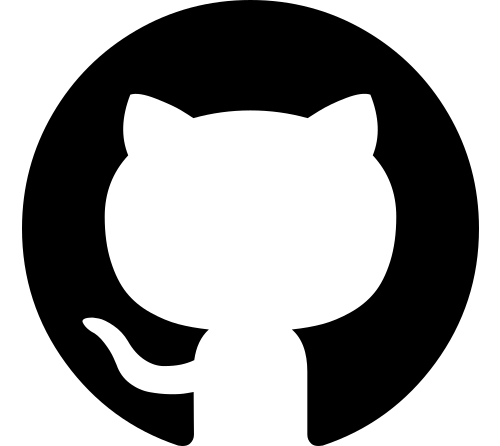
\includegraphics[height=.05\textheight]{resources/github-icon.png}} 
\includegraphics[height=.05\textheight]{resources/slack-icon.png} ComicSansMS

    \item \href{https://twitter.com/DerGhulbus/}{
\includegraphics[height=.05\textheight]{resources/twitter-icon.png} @DerGhulbus}

    \item 
\includegraphics[height=.05\textheight]{resources/meetup-icon.png} Co-organizer of the \href{https://www.meetup.com/MUCplusplus/}{Munich C++ User Group}

    \item Currently working as a Software Architect for BMW 
\includegraphics[height=.1\textheight]{resources/bmw_group.jpg}

  \end{itemize}
\end{frame}
\fi


\begin{frame}[fragile]
%  \frametitle{The Problem}

  \begin{center}
    \Huge \texttt{-fno-exceptions}
  \end{center}
\end{frame}

\iffalse
\begin{frame}[fragile]

  \frametitle{The Problem}
  
  \begin{lstlisting}
class Foo {
private:
  std::unique_ptr<InternalState> m_state;  
public:
  Foo(Arg n_arg)
  :m_state(std::make_unique<InternalState>(n_arg))
  { }
};
  \end{lstlisting}
  
\end{frame}
\fi

\begin{frame}[fragile]

  \frametitle{The Problem}
  
  \begin{semiverbatim}
{\color{blue}class} Foo \{
{\color{blue}private}:
  std::unique_ptr<InternalState> m_state;  
{\color{blue}public}:
  Foo(Arg n_arg)
  :m_state(std::make_unique<InternalState>(n_arg))
  \{ \}
\};
  \end{semiverbatim}
  
\end{frame}


\begin{frame}[fragile]

  \frametitle{The Problem}
  
  \begin{semiverbatim}
{\color{blue}class} Foo \{
{\color{blue}private}:
  std::unique_ptr<InternalState> m_state;  
{\color{blue}public}:
  Foo(Arg n_arg)
  :m_state({\color{red}std::make_unique<InternalState>(n_arg)})
  \{ \}
\};
  \end{semiverbatim}
  
\end{frame}


\begin{frame}[fragile]

  \frametitle{Two-Phase Initialisation}
  
  \begin{semiverbatim}
{\color{blue}class} Foo \{
{\color{blue}private}:
  std::unique_ptr<InternalState> m_state;  
{\color{blue}public}:
  Foo() {\color{blue}noexcept}
  :m_state()
  \{ \}
\};
  \end{semiverbatim}
  
\end{frame}


\begin{frame}[fragile]

  \frametitle{Two-Phase Initialisation}
  
  \begin{semiverbatim}
{\color{blue}class} Foo \{
{\color{blue}private}:
  std::unique_ptr<InternalState> m_state;  
{\color{blue}public}:
  Foo() {\color{blue}noexcept}
  :m_state()
  \{ \}






\};
  \end{semiverbatim}
  
\end{frame}


\begin{frame}[fragile]

  \frametitle{Two-Phase Initialisation}
  
  \begin{semiverbatim}
{\color{blue}class} Foo \{
{\color{blue}private}:
  std::unique_ptr<InternalState> m_state;  
{\color{blue}public}:
  Foo() {\color{blue}noexcept}
  :m_state()
  \{ \}

  std::error_code init(Arg n_arg) {\color{blue}noexcept} \{
    {\color{red}m_state = make_unique_nothrow(n_arg);}


  \}
\};
  \end{semiverbatim}
  
\end{frame}



\begin{frame}[fragile]

  \frametitle{Two-Phase Initialisation}
  
  \begin{semiverbatim}
{\color{blue}class} Foo \{
{\color{blue}private}:
  std::unique_ptr<InternalState> m_state;  
{\color{blue}public}:
  Foo() {\color{blue}noexcept}
  :m_state()
  \{ \}

  std::error_code init(Arg n_arg) {\color{blue}noexcept} \{
    m_state = make_unique_nothrow(n_arg);
    {\color{blue}if}(!m_state) \{ {\color{blue}return} \{ my_errc::error, my_category() \}; \}
    {\color{blue}return} std::error_code();
  \}
\};
  \end{semiverbatim}
  
\end{frame}


\begin{frame}
  \begin{itemize}
  \item Objects in partial constructed state
  \end{itemize}
\end{frame}


\begin{frame}[fragile]

  \frametitle{A first attempt to fix this\ldots}
  
  \begin{semiverbatim}
{\color{blue}class} Foo \{
{\color{blue}private}:
  std::unique_ptr<InternalState> m_state;  
{\color{blue}public}:
  Foo() {\color{blue}noexcept}
  :m_state()
  \{ \}

  std::error_code init(Arg n_arg) {\color{blue}noexcept} \{
    m_state = make_unique_nothrow(n_arg);
    {\color{blue}if}(!m_state) \{ {\color{blue}return} \{ my_errc::error, my_category() \}; \}
    {\color{blue}return} std::error_code();
  \}
\};
  \end{semiverbatim}
  
\end{frame}


\begin{frame}[fragile]

  \frametitle{A first attempt to fix this\ldots}

  \begin{semiverbatim}
{\color{blue}class} Foo \{
{\color{blue}private}:
  std::unique_ptr<InternalState> m_state;  

  Foo() {\color{blue}noexcept}
  :m_state()
  \{ \}
{\color{red}public}:
  std::error_code init(Arg n_arg) {\color{blue}noexcept} \{
    m_state = make_unique_nothrow(n_arg);
    {\color{blue}if}(!m_state) \{ {\color{blue}return} \{ my_errc::error, my_category() \}; \}
    {\color{blue}return} std::error_code();
  \}
\};
  \end{semiverbatim}
  
\end{frame}



\begin{frame}[fragile]

  \frametitle{A first attempt to fix this\ldots}

  \begin{semiverbatim}
{\color{blue}class} Foo \{
{\color{blue}private}:
  std::unique_ptr<InternalState> m_state;  
  Foo() {\color{blue}noexcept}
  :m_state()
  \{ \}
{\color{blue}public}:
  {\color{red}static expected<Foo> create}(Arg n_arg) {\color{blue}noexcept} \{




  \}
\};
  \end{semiverbatim}  
\end{frame}

\begin{frame}[fragile]

  \frametitle{A first attempt to fix this\ldots}

  \begin{semiverbatim}
{\color{blue}class} Foo \{
{\color{blue}private}:
  std::unique_ptr<InternalState> m_state;  
  Foo() {\color{blue}noexcept}
  :m_state()
  \{ \}
{\color{blue}public}:
  {\color{blue}static} expected<Foo> create(Arg n_arg) {\color{blue}noexcept} \{
    Foo ret\{\};
    ret.m_state = make_unique_nothrow(n_arg);
    {\color{blue}if}(!ret.m_state) \{ {\color{blue}return} unexpected(my_errc::error); \}
    {\color{blue}return} ret;
  \}
\};
  \end{semiverbatim}  
\end{frame}


\begin{frame}
  \begin{itemize}
  \item \sout{Objects in partial constructed state} \checkmark
    \pause
  \item {\color{red}Non-idiomatic construction}
  \end{itemize}
\end{frame}


\begin{frame}[fragile]

  \frametitle{Inverse Two-Phase Initialisation}

  \begin{semiverbatim}
{\color{blue}static} expected<Foo>
    create(Arg n_arg) {\color{blue}noexcept}
\{
  Foo ret{};
  ret.m_state = make_unique_nothrow(n_arg);
  {\color{blue}if}(!ret.m_state) \{ {\color{blue}return} unexpected(my_errc::error); \}
  {\color{blue}return} ret;
\}

  \end{semiverbatim}  
\end{frame}


\begin{frame}[fragile]

  \frametitle{Inverse Two-Phase Initialisation}

  \begin{semiverbatim}
{\color{blue}static} expected<{\color{red}construction_token}>
    {\color{red}preconstruct}(Arg n_arg) {\color{blue}noexcept}
\{
  {\color{red}construction_token} t;
  t.state = make_unique_nothrow(n_arg);
  {\color{blue}if}(!t.state) \{ {\color{blue}return} unexpected(my_errc::error); \}
  {\color{blue}return} t;
\}




  
  \end{semiverbatim}  
\end{frame}


\begin{frame}[fragile]

  \frametitle{Inverse Two-Phase Initialisation}

  \begin{semiverbatim}
{\color{blue}static} expected<construction_token>
    preconstruct(Arg n_arg) {\color{blue}noexcept}
\{
  construction_token t;
  t.state = make_unique_nothrow(n_arg);
  {\color{blue}if}(!t.state) \{ {\color{blue}return} unexpected(my_errc::error); \}
  {\color{blue}return} t;
\}

Foo(construction_token&& t) {\color{blue}noexcept}
:m_state(std::move(t.state))
\{ \}
  
  \end{semiverbatim}  
\end{frame}



\begin{frame}[fragile]

  \frametitle{Inverse Two-Phase Initialisation (User's view)}

  \begin{semiverbatim}
    {\color{blue}auto} t1 = Foo::preconstruct(args);
    Foo obj(std::move(t1));
\pause    
    {\color{gray} \textit{// or}}
    {\color{blue}auto} t2 = Foo::preconstruct(args);
    {\color{blue}auto} obj_ptr = std::make_shared<Foo>(std::move(t2));
    \pause
    {\color{gray} \textit{// or}}
    {\color{blue}auto} t3 = Foo::preconstruct(args);
    std::vector<Foo> objects;
    objects.emplace_back(std::move(t3));
  \end{semiverbatim}  
\end{frame}


\begin{frame}
  \begin{itemize}
  \item \sout{Objects in partial constructed state} \checkmark
  \item \sout{Non-idiomatic construction} \checkmark
  \end{itemize}
\end{frame}


\begin{frame}[fragile]

  \frametitle{Inverse Two-Phase Initialisation}

  \begin{semiverbatim}
{\color{blue}static} expected<construction_token>
    preconstruct(Arg n_arg) {\color{blue}noexcept}
\{
  construction_token t;
  t.state = make_unique_nothrow(n_arg);
  {\color{blue}if}(!t.state) \{ {\color{blue}return} unexpected(my_errc::error); \}
  {\color{blue}return} t;
\}

Foo(construction_token&& t) {\color{blue}noexcept}
:m_state(std::move(t.state))
\{ \}
  
  \end{semiverbatim}  
\end{frame}


\end{document}
